\documentclass{article}
\usepackage{graphicx} % Required for inserting images
\usepackage{float}
\usepackage{parskip}
\usepackage{hyperref}
\usepackage{url} % Better URL handling
\urlstyle{same} % Use the same font for URLs
\usepackage{apacite}
\usepackage{enumitem} % For nested lists in maze generation section
\usepackage[margin=1.5in]{geometry} % Reduce horizontal padding
\usepackage{tikz} % For creating plots and diagrams
\usepackage{pgfplots} % For creating plots
\pgfplotsset{compat=1.18} % Set compatibility level

\title{Simple Doom Game Clone in Three.js}
\author{Elias Nijs \& René Van Der Schueren}
\date{May 2025}

% Custom title page information
\newcommand{\courseinfo}{Computer Graphics (E016712A)}
\newcommand{\academicyear}{Academic Year 2024/2025}
\newcommand{\university}{GHENT UNIVERSITY}

\begin{document}

% Custom title page
\begin{titlepage}
    \centering
    \vspace*{1cm}
    
    \Huge
    \textbf{Simple Doom Game Clone in Three.js}\\
    \vspace{1.5cm}
    
    \Large
    \textbf{\courseinfo}\\
    \vspace{0.5cm}
    
    \large
    \university\\
    \vspace{0.5cm}
    
    \vspace{1.5cm}
    
    \Large
    Elias Nijs \& René Van Der Schueren\\
    \vspace{0.5cm}
    
    \large
    \academicyear\\
    \vspace{0.5cm}
    
    \large
    May 2025\\
    
\end{titlepage}

\pagebreak

\tableofcontents

\pagebreak

\begin{figure}[H]
    \centering
    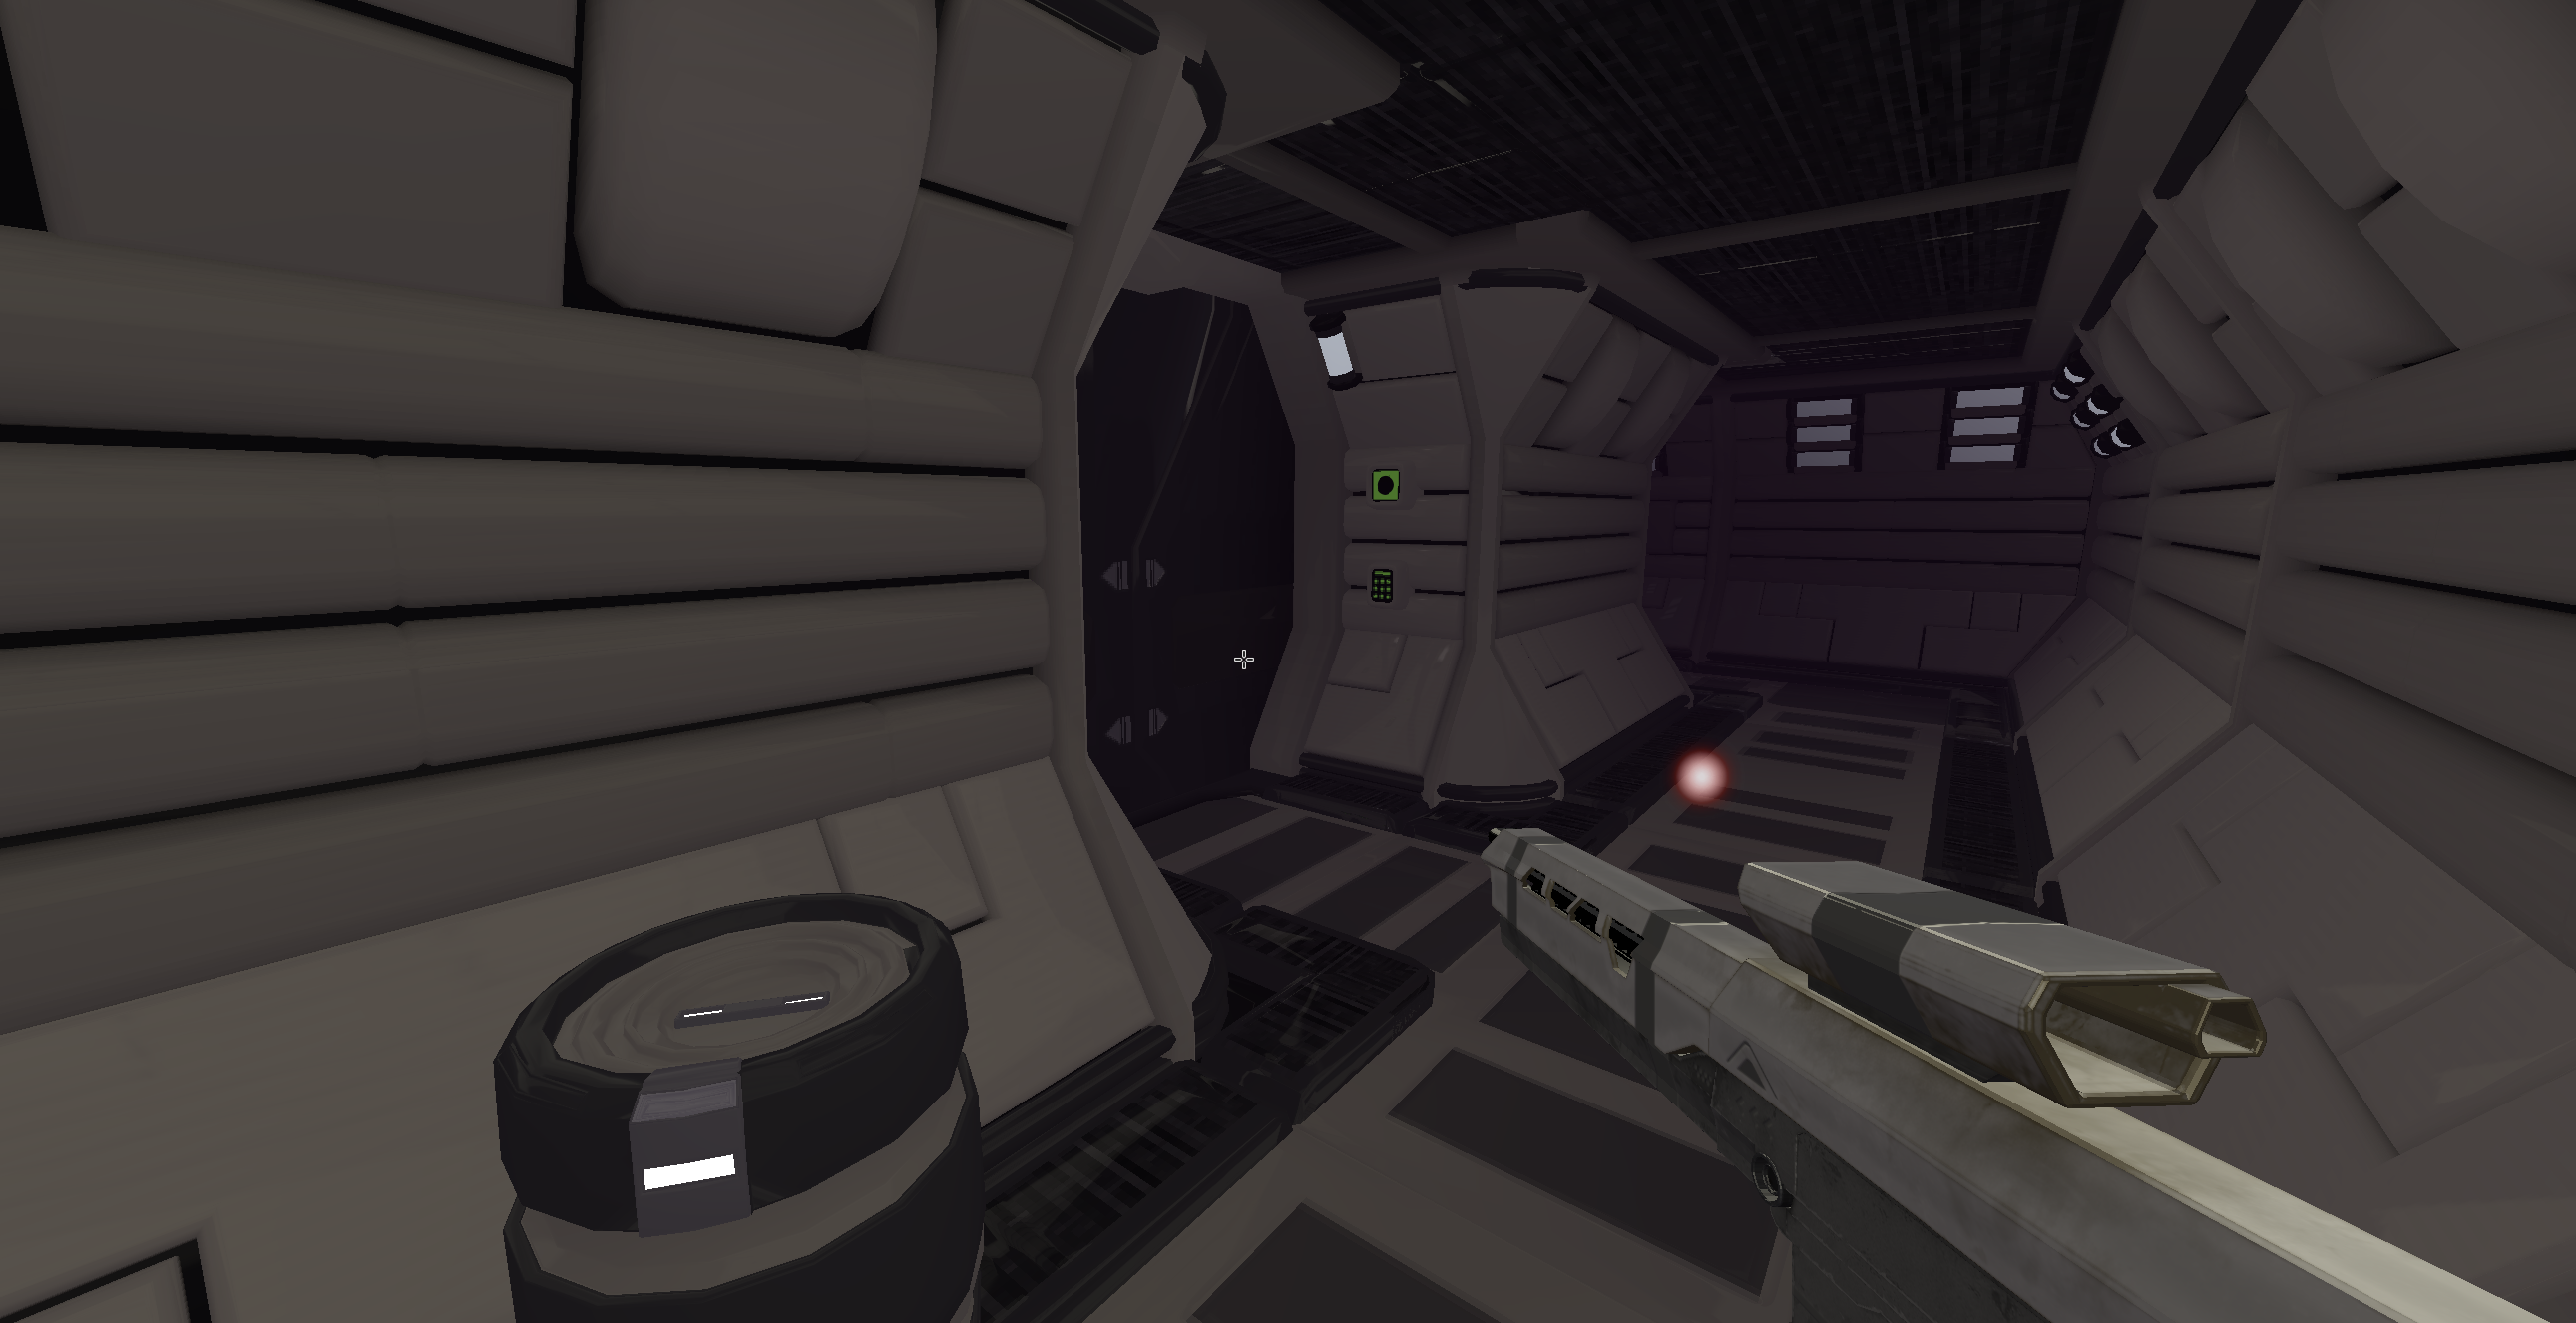
\includegraphics[width=\textwidth]{diagrams/gameplay.png}
    \caption{Gameplay screenshot of our Doom-inspired game implemented in Three.js.}
    \label{fig:gameplay-main}
\end{figure}

\section{Introduction}\label{sec:introduction}
\subsection{Tech Choices}
Our project uses Three.js, a lightweight JavaScript library that abstracts WebGL for accessible 3D graphics programming in browsers. We chose it for its robust ecosystem, documentation, and optimized web rendering performance. Development is powered by Vite for fast server capabilities, and we implemented the codebase in TypeScript to benefit from static typing, which improves code reliability and facilitates better team collaboration.

\subsection{Gameplay Overview}
Our game is a first-person shooter inspired by the classic Doom, implemented using Three.js. Players navigate through procedurally generated mazes, interact with doors, follow path markers, and encounter various props while trying to reach their destination. Players can also shoot their gun to open doors, adding a combat element to the navigation mechanics.

\begin{figure}[H]
    \centering
    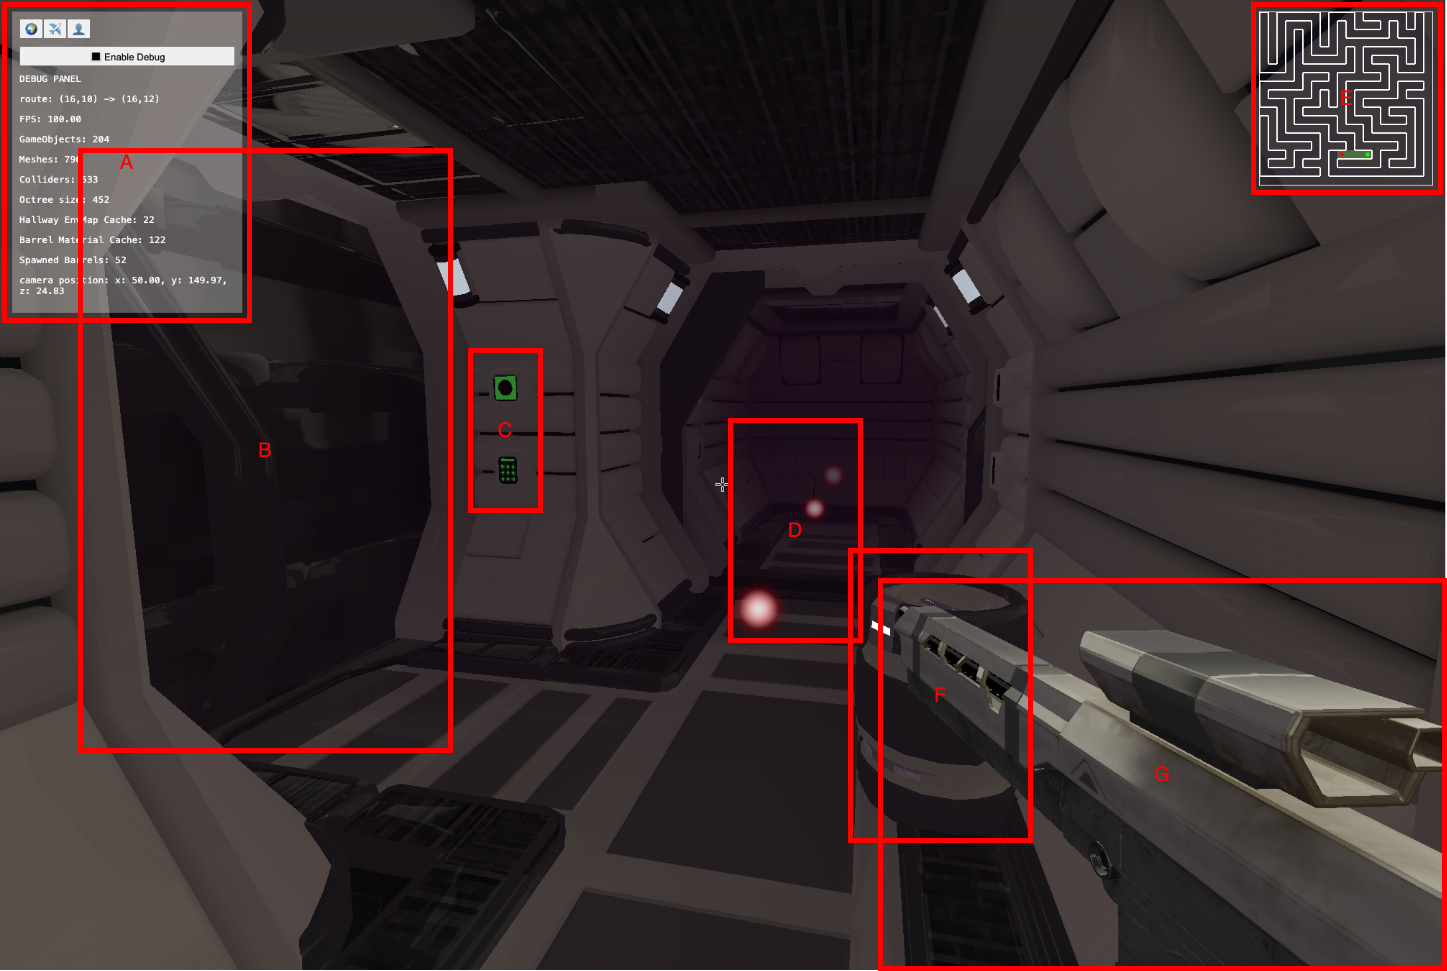
\includegraphics[width=\textwidth]{diagrams/screenshot.png}
    \caption{Gameplay screenshot showing key elements: (A) Debug menu for adjusting game parameters, (B) Closed door with its control panel (C), (D) Path markers guiding the player through an open door, (E) Mini-map displaying player position and path to destination, (F) Barrel spawned as a random prop, and (G) Weapon in gun mode.}
    \label{fig:gameplay-overview}
\end{figure}

Figure \ref{fig:gameplay-overview} illustrates the main gameplay elements:
\begin{itemize}
    \item \textbf{A:} Debug menu that allows changing camera settings, enabling debug mode, and displays game engine statistics.
    \item \textbf{B:} A door that was previously opened, allowing passage through the maze.
    \item \textbf{C:} Door control panel that can be activated by shooting it with the player's weapon.
    \item \textbf{D:} Path markers showing the optimal route to the destination, guiding the player through an open door.
    \item \textbf{E:} Mini-map displaying the player's current position in red,  and the path to the destination, marked in green.
    \item \textbf{F:} Barrel that was procedurally spawned as a random prop in the environment.
    \item \textbf{G:} The player's weapon in gun mode.
\end{itemize}


\section{Game Engine}
Before diving into specific features, we'll provide an overview of our custom game engine architecture that powers the entire application.

\subsection{Core Architecture}
Our game engine follows a component-based design pattern, with a central state management system that coordinates all game elements. The engine is structured around these key components:

\begin{itemize}
    \item \texttt{GameObject}: An abstract base class that serves as the foundation for all entities in the game world. Each game object automatically registers itself with the state management system upon creation and implements lifecycle methods such as \texttt{animate} (called every frame), \texttt{cleanup}, and \texttt{destroy}.
    
    \item \texttt{State}: The central management class that maintains references to all active game objects, handles scene configuration, manages the camera system, and coordinates the physics simulation. It provides methods for registering and unregistering game objects, finding objects by type, toggling debug visualization, ...
    
    \item \texttt{Physics}: A collision detection and resolution system that uses axis-aligned bounding boxes (AABBs) to represent object boundaries. The physics system calculates collision corrections and applies them to maintain proper object separation. For efficient collision detection, we implemented an octree-based spatial partitioning system (explained in detail in the Space Partitioning section), which significantly reduces the number of collision checks by organizing objects hierarchically based on their spatial location.
\end{itemize}

\subsection{Game Loop}
The engine implements a standard game loop that:

\begin{enumerate}
    \item Calls the \texttt{animate} method on the state, which in turn calls all registered game objects.
    \item Updates the physics system and rebuilds the dynamic octree.
    \item Renders the scene.
\end{enumerate}

This architecture provides a solid foundation for implementing the game-specific features described in the following sections.

\section{Maze Generation}
First, we will start by explaining our maze generation algorithm, which forms the foundation of our game's level design.

\subsection{Implementation}

The maze generation system is implemented as a modular component in the utils directory. It provides function for creating the abstract maze structure but not for converting it to the physical 3D environment. This separation of concerns allows the maze logic to be tested independently from the game rendering system while maintaining a clean integration between the two.

\subsubsection{Data Structures}
The maze is represented by a grid of cells, where each cell contains information about its walls and visited state:
\begin{itemize}
    \item \texttt{Cell}: A type representing a single cell in the maze with properties for walls (north, east, south, west) and a visited flag.
    \item \texttt{Grid}: A type containing an array of cells and dimensions (number of rows and columns).
    \item \texttt{Pos}: A type alias for a position in the grid, represented as [row, column].
\end{itemize}

\subsubsection{Generation Algorithm}
The maze generation follows these steps:
\begin{enumerate}
    \item Initialize a grid where all cells have all four walls intact and are marked as unvisited.
    \item Start at a cell (typically [0,0]) and mark it as visited.
    \item Push the starting cell onto a stack to track the path.
    \item While the stack is not empty:
    \begin{enumerate}
        \item Get the current cell from the top of the stack.
        \item If the current cell has any unvisited neighbors:
        \begin{enumerate}
            \item Choose one randomly.
            \item Remove the wall between the current cell and the chosen neighbor.
            \item Mark the neighbor as visited.
            \item Push the neighbor onto the stack.
        \end{enumerate}
        \item If there are no unvisited neighbors, pop the current cell from the stack (backtrack).
    \end{enumerate}
\end{enumerate}

This algorithm ensures that every cell in the maze is reachable from any other cell, creating a perfect maze with exactly one path between any two points.

\subsubsection{Upscaling}
The implementation includes an optional upscaling feature that doubles the effective resolution of the maze by inserting buffer cells between the original cells. This creates a more visually appealing maze with wider corridors while maintaining the logical structure of the original maze. Additionally, the upscaling process leaves room between parallel hallways, providing space for game elements such as doors to animate into when opened, enhancing the interactive experience without causing clipping or collision issues. Figure \ref{fig:maze-spacing} illustrates the difference between a maze without spacing and one with spacing, clearly showing how the upscaling creates buffer zones between parallel corridors.

\begin{figure}[H]
    \centering
    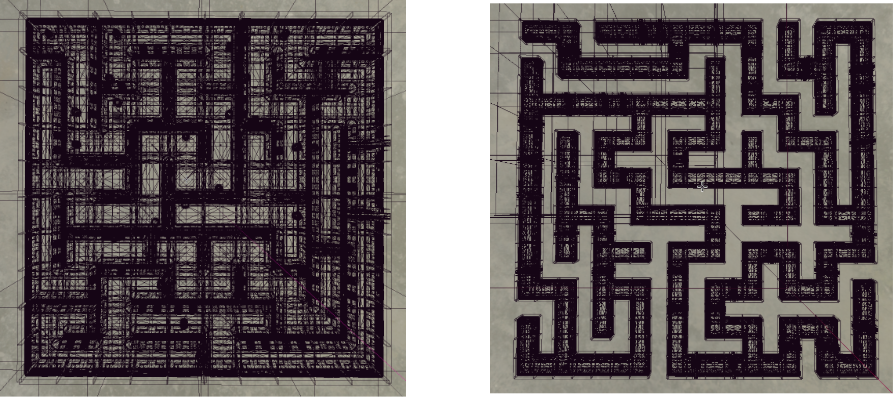
\includegraphics[width=0.8\textwidth]{diagrams/spacing.png}
    \caption{Comparison of a 10x10 maze: left without spacing, right with spacing, viewed from the top in debug mode. Notice the extra spacing making sure that parallel hallways do not touch.}
    \label{fig:maze-spacing}
\end{figure}

\subsubsection{Pathfinding}
The implementation features an efficient A* pathfinding algorithm that calculates optimal routes between any two points in the maze. This algorithm employs a Manhattan distance heuristic—particularly suitable for grid-based movement—and accounts for walls when evaluating potential paths. The pathfinding system provides visual guidance for players through path markers that highlight the shortest route to objectives. The algorithm maintains separate data structures for tracking both the cost of the path so far (g-score) and the estimated total cost to the destination (f-score), ensuring optimal path discovery even in complex maze configurations.


\section{3D World Organization}
Our 3D world uses a modular approach with standardized hallway units as building blocks, optimizing both performance and visual quality.

The world is built on a grid of uniform hallway segments, each occupying one grid cell with consistent dimensions. Hallways have identical outer dimensions with internal variations (straight, corner, junction) and are positioned using precise grid coordinates. While hallway elements are hierarchically organized in the Three.js scene, our GameObject system maintains a flat structure for efficient game logic.

Our system loads all hallway variants from a single GLB file and clones meshes rather than creating new geometry for each instance. Materials and environment maps are cached to prevent redundant creation. This approach significantly reduces memory usage and draw calls, enabling efficient rendering of large mazes.

The player exists as a separate entity from the environment structure, comprising a first-person camera at eye level, a weapon model in the lower view portion, collision geometry for physical interaction, and independent movement and interaction logic. The player navigates through the hallway grid using keyboard and mouse controls, with collision detection preventing movement through walls and other obstacles. The camera's position and orientation update in real-time based on player input, creating a smooth first-person experience.

Our world features several dynamic elements: sliding doors that update collision geometry in real-time; interactive door control panels; sprite-based path markers; procedurally distributed props; and temporary bullet impact markers that fade over time to maintain performance while providing visual feedback (see Figure~\ref{fig:bullet-markers}). All these elements—doors, control panels, props, and other interactive objects—are implemented as children of their respective hallway parts in the scene hierarchy, maintaining a clean organizational structure while preserving the flat GameObject system for game logic.

\begin{figure}[H]
    \centering
    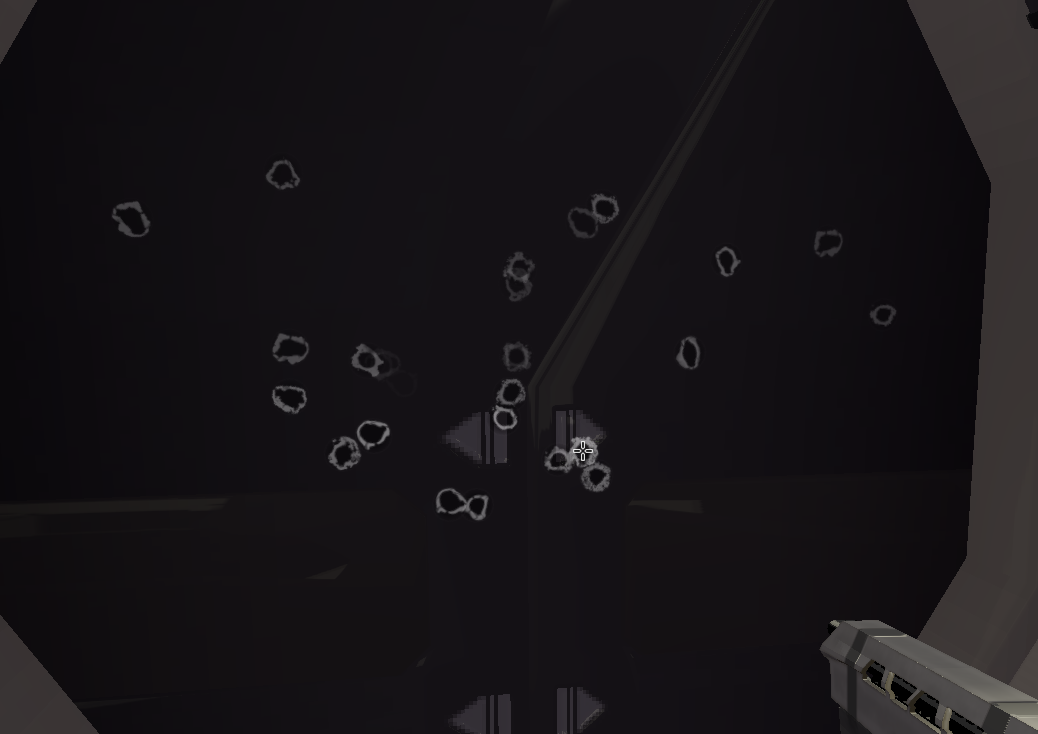
\includegraphics[width=0.6\textwidth]{diagrams/bullets.png}
    \caption{Bullet impact markers on walls that gradually fade over time and are eventually deleted to conserve resources, providing visual feedback of weapon impacts while maintaining performance.}
    \label{fig:bullet-markers}
\end{figure}


\section{User Controls and Movement}
Our Doom clone implements a classic first-person shooter control scheme. Player movement is controlled using the WASD keys, with W and S for forward and backward movement, and A and D for strafing left and right. Mouse input controls the camera rotation, allowing players to look around the environment with configurable sensitivity parameters.

The movement system applies the player's directional input to a normalized vector, which is then rotated according to the player's current view direction. This creates the expected behavior where pressing W always moves the player forward relative to their view. Movement velocity is controlled by adjustable speed parameters and is framerate-independent thanks to delta time scaling.Collision detection prevents the player from moving through walls, this is explained later.

The game also features immersive visual feedback during movement, with a weapon bob animation that simulates the natural motion of carrying a weapon while walking. This is achieved by applying sinusoidal oscillations to the weapon position based on the player's movement state. Additionally, the weapon model automatically lowers when the player approaches a wall, providing a realistic response to close-proximity obstacles and preventing clipping issues.

\section{Lighting, Materials and Texture Mapping}
TODO

\section{Collision Detection Using Octree}

For efficient collision detection in our 3D game environment, we implemented an octree-based spatial partitioning system that significantly reduces the computational complexity of detecting object interactions.

\subsection{Octree Implementation}
Our implementation uses a standard octree data structure with several
optimizations for performance and memory efficiency. The octree stores
colliders directly in a list, with the nodes of the octree itself storing
indices into this list rather than the actual collider objects. This approach
allows multiple octree nodes to reference the same collider without
duplication.

When inserting a collider into the octree, its indices are spread over all
partitions that overlap with the bounding box of the element, ensuring that
queries will find colliders that span multiple octants. For efficient octant
determination, we use bit patterns to index the octree, leveraging the
isomorphism between 3 bits and the 8 octants of the tree. This binary
representation allows for quick computation of which octant a point belongs to.

To prevent excessive subdivision in dense areas, our implementation enforces a maximum depth limit for the octree. This constraint ensures that the tree doesn't become too deep in areas with many colliders, which would otherwise lead to diminishing returns in performance and increased memory usage. The maximum depth was determined experimentally to balance the tradeoff between query performance and memory consumption, with a value that provides optimal performance for our game's typical scenes.

For memory management, we optimize removal operations by marking elements as
dead in the backing list rather than physically removing them. This approach
avoids costly array operations and simplifies the tree maintenance logic.

\subsubsection{Computational Complexity}
The octree provides significant performance advantages over naive collision detection approaches, with the following complexity characteristics:

\begin{itemize}
    \item \textbf{Construction}: Building the octree has a complexity of $O(n \log n)$ in the average case, where $n$ is the number of colliders. Each insertion operation takes $O(\log n)$ time as it traverses down the tree to place the collider in the appropriate nodes.
    
    \item \textbf{Query}: Collision queries achieve an average-case complexity of $O(\log n + k)$, where $k$ is the number of colliders in the vicinity of the query. This is substantially better than the $O(n)$ complexity of brute-force approaches that check against every collider in the scene.
    
    \item \textbf{Memory}: The octree's space complexity is $O(n)$ in the average case, but can approach $O(n^2)$ in the worst case when many colliders span multiple octants, requiring multiple references in the tree.
\end{itemize}

In practice, our implementation maintains near-logarithmic performance for most game scenes, with degradation only occurring in extremely dense environments where many objects overlap significantly. The practical benefits of our octree implementation are quantified in the benchmarks presented in Section \ref{sec:benchmarking}, where we demonstrate how this spatial partitioning approach enables consistent frame rates even with increasing scene complexity.

\subsection{Engine Integration}
Our game engine maintains two separate octrees: one for static objects (walls,
floors, stationary props) and another for dynamic objects (player, moving
doors, projectiles). This separation optimizes performance since the static
tree never changes after level initialization and thus never needs to be
rebuilt, while the dynamic tree is rebuilt each frame to account for moving
objects.

Game objects are responsible for managing their own colliders and must register
or unregister them with the state management system. The registration process
includes a flag to specify whether the collider should be added to the static
or dynamic tree, giving developers fine-grained control over collision
behavior.

For debugging purposes, we implemented a visualization system that renders the
octree structure with color coding based on depth. Deeper nodes are displayed
in blue while shallower nodes are displayed in red, with varying opacity to
enhance visibility. This visualization has been invaluable for debugging
spatial partitioning issues and understanding collision behavior in complex
scenes.

\subsection{Collision Resolution}
Since our game world is organized on a grid, we use axis-aligned bounding boxes
(AABBs) as colliders for all game objects. When checking for collisions, we
query both the static and dynamic octrees to retrieve all colliders that share
the same spatial partition as the object being tested.

Our collision resolution algorithm implements several sophisticated techniques:

First, we determine the amount of overlap between colliding objects in the
direction of movement. The system then implements minimum penetration axis
selection by comparing overlaps in the X, Y, and Z directions and only applying
correction along the axis with the smallest overlap. This approach, based on
the separating axis theorem, ensures that objects are pushed apart along the
most efficient path.

The algorithm employs direction-aware displacement, determining the sign of the
correction based on the relative position of collider centers. This ensures
that objects are always pushed in the correct direction to separate them,
regardless of their relative positions or movement directions.

For handling multiple simultaneous collisions, we accumulate displacement
vectors from all collisions and track how many meaningful collisions occurred
(ignoring zero-displacement cases). The accumulated vector is then scaled by a
factor of 1.1 to add a small push-out buffer that prevents objects from getting
stuck at the exact collision boundary. Finally, the displacement is averaged by
dividing by the number of collisions, creating a balanced response that
prevents erratic movement when multiple collisions occur.

Our system calculates the direction of the displacement vectors using the
centers of bounding boxes rather than object positions directly. This
center-based direction calculation provides more reliable and consistent
collision responses, especially for objects with offset centers or irregular
shapes represented by AABBs.


\section{Benchmarking}\label{sec:benchmarking}
To assess the performance and efficiency of our implementation, we conducted a series of controlled tests focusing on key areas that affect gameplay and user experience. These benchmarks provide quantitative data on how our design choices impact performance as scale increases, helping to identify optimization opportunities and hardware requirements.

\subsection{Maze Size Performance Analysis}
To evaluate the scalability of our implementation, we conducted performance tests with mazes of increasing size. All tests were performed on a MacBook Air (2022) with an Apple M2 chip, 8-core CPU, 8-core GPU, and 24GB of unified memory. The performance was measured in frames per second (FPS) while maintaining all graphical settings and game features at consistent levels.

Table \ref{tab:maze-performance} presents the relationship between maze dimensions, scene complexity (measured by the number of game objects and meshes), and rendering performance. The maze dimensions represent the logical grid size before upscaling, while the total tiles indicate the actual number of navigable cells in the generated maze.

\begin{table}[H]
    \centering
    \begin{tabular}{|c|c|c|c|c|}
        \hline
        \textbf{Maze Size} & \textbf{Total Tiles} & \textbf{Game Objects} & \textbf{Mesh Count} & \textbf{FPS} \\ \hline
        10×10 & 100 & 204 & 697 & 100 \\ \hline
        20×20 & 400 & 904 & 2,844 & 100 \\ \hline
        40×40 & 1,600 & 3,204 & 11,595 & 50 \\ \hline
        80×80 & 6,400 & 12,804 & 46,477 & 10 \\ \hline
        160×160 & 25,600 & 51,204 & 187,113 & 2.5 \\ \hline
    \end{tabular}
    \caption{Performance metrics for different maze sizes showing the relationship between maze dimensions, scene complexity, and frame rate.}
    \label{tab:maze-performance}
\end{table}

\begin{figure}[H]
    \centering
    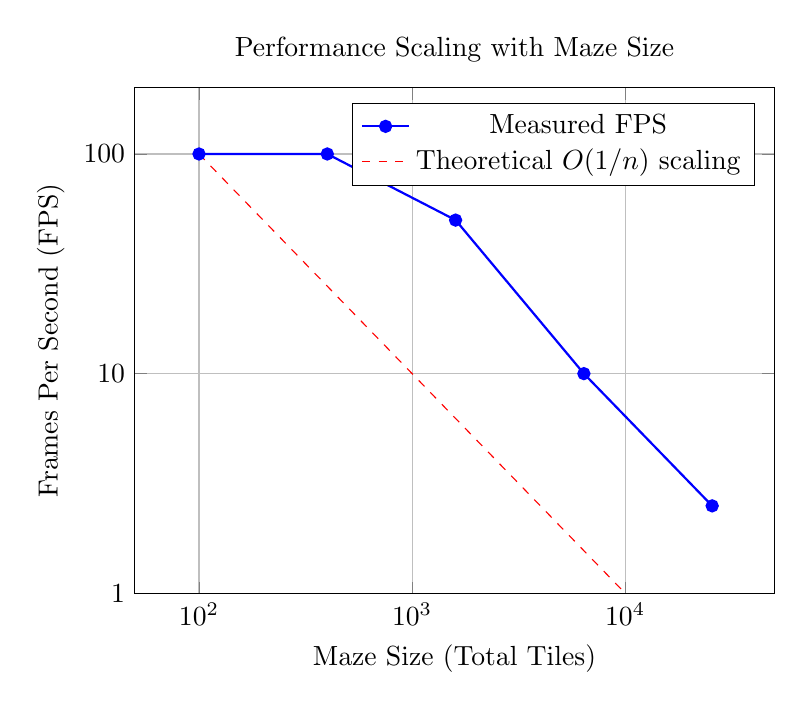
\begin{tikzpicture}
    \begin{axis}[
        width=0.8\textwidth,
        height=8cm,
        xlabel={Maze Size (Total Tiles)},
        ylabel={Frames Per Second (FPS)},
        xmode=log,
        ymode=log,
        log basis x=10,
        log basis y=10,
        grid=both,
        legend pos=north east,
        xmin=50, xmax=50000,
        ymin=1, ymax=200,
        xtick={100,1000,10000},
        xticklabels={$10^2$,$10^3$,$10^4$},
        ytick={1,10,100},
        yticklabels={1,10,100},
        title={Performance Scaling with Maze Size}
    ]
    
    % FPS vs Total Tiles data points
    \addplot[color=blue,mark=*,thick] coordinates {
        (100, 100)
        (400, 100)
        (1600, 50)
        (6400, 10)
        (25600, 2.5)
    };
    
    % Theoretical inverse relationship curve (1/x)
    \addplot[color=red,dashed,domain=100:25600,samples=100] {10000/x};
    
    \legend{Measured FPS, Theoretical $O(1/n)$ scaling}
    \end{axis}
    \end{tikzpicture}
    \caption{Log-log plot showing the relationship between maze size (total tiles) and performance (FPS). The dashed red line represents theoretical inverse scaling, demonstrating how our implementation closely follows expected performance characteristics as scene complexity increases.}
    \label{fig:performance-scaling}
\end{figure}

As evident from the data, our implementation maintains an optimal frame rate of 100 FPS for mazes up to 20×20 (400 tiles), demonstrating that the game is well-optimized for small to medium-sized environments. Note that the 100 FPS ceiling is due to the testing monitor's maximum refresh rate; the actual performance for smaller mazes may exceed this value. Performance begins to degrade at 40×40 (1,600 tiles), dropping to 50 FPS, which is still playable but shows the increasing computational demands.

At the extreme end, the 160×160 maze (containing 25,600 tiles and over 187,000 meshes) pushes the hardware to its limits, resulting in only 5 FPS. While not playable, this test demonstrates the upper bounds of our implementation on consumer hardware and provides valuable insights for future optimization efforts.

\subsection{Octree}

\pagebreak
\section{Art Credits}
While the focus of this project was on the technical implementation of computer graphics concepts, we utilized several third-party 3D models and textures to enhance the visual quality of our game. All assets were used under appropriate licenses, and modifications were made to better suit our game's aesthetic and technical requirements.

\begin{itemize}
    \item \textbf{Hallway Modules}: The modular hallway system was based on assets from "Spaceship Modules" by ThisIsBranden, available at \url{https://thisisbranden.itch.io/spaceship-modules}.
    
    \item \textbf{Environmental Props}: Various props such as barrels and crates were sourced from the "Sci-Fi Assets Pack" available on TurboSquid at \url{https://www.turbosquid.com/3d-models/sci-fi-assets-model-1876664}.
    
    \item \textbf{Weapon Model}: The player's gun was adapted from the "Sci-Fi DMR" model available on TurboSquid at\\\url{https://www.turbosquid.com/3d-models/3d-scifi-dmr-model-1983451}.
\end{itemize}

Small modifications were made to these models using Blender. Texture adjustments were performed using Krita. This was done to maintain a consistent visual style throughout the game environment.

% \pagebreak
% \nocite{*}
% \bibliographystyle{apacite}
% \bibliography{references}

\end{document}
